\section{Choosing integers that do not share primes}\label{fin:selection}
Put the integers $2,3,\ldots,X$ on cards.  We may keep as many cards
as we like, provided no two kept cards share a prime factor.
Thus $8$ and $9$ can sit together; $6$ and $10$ cannot.
The prime $2$ is a resource that the second pair tries to spend twice.

Now choose an admissible collection uniformly at random.
How many cards does it contain?  The cards interact in a complicated
way, but the answer is almost the size of a pile of independent fair
coin flips.  Better still, an independent binomial part can be extracted
\emph{exactly}, before taking any limit.

\subsection{A small example with a coin inside}
For the five cards $2,3,4,5,6$, the admissible collections have
generating polynomial
\[
 1+5z+6z^2+2z^3=(1+z)(1+4z+2z^2).
\]
The coefficient of $z^j$ counts the collections of size $j$.
There are fourteen collections in all, including the empty one.
The factor $1+z$ has an immediate explanation: the card $5$ shares
no prime with any other card, so it can be added or removed freely.
A uniformly chosen collection therefore contains this card according
to an independent fair coin.

For a larger interval the free coins need not have fixed names.
Choosing a composite card may use up prime cards that would otherwise
be available.  Nevertheless, a large binomial component survives in
the \emph{distribution of the number of cards kept}.

To include later deletion experiments, let $B$ be any set of allowed
primes.  Write $\mathcal N_B(X)$ for the integers in $[2,X]$ whose
prime divisors all belong to $B$, and define
\[
 P_{B,X}(z)=\sum_{\substack{S\subseteq\mathcal N_B(X)\\
                       S\ {\rm pairwise\ coprime}}}z^{|S|}.
\]
Here $N_B=\#(B\cap[2,X])$ counts available prime cards,
$r_B=\#(B\cap[2,\sqrt X])$ counts the small ones, and
\[
 m_B=\max(0,N_B-2r_B),\qquad d_B=N_B-m_B.
\]
\begin{theorem}[The binomial component]\label{fin:binomial}
There is a polynomial $Q_{B,X}$ with nonnegative integer coefficients,
of degree $d_B$, such that
\[
 \boxed{P_{B,X}(z)=(1+z)^{m_B}Q_{B,X}(z).}
\]
Give each admissible subset probability proportional to
$\lambda^{|S|}$, where $\lambda>0$, and put
$\theta=\lambda/(1+\lambda)$.  Its size has the exact distribution
\begin{equation}
 |S|\ \overset d=\ Z+R,\qquad
 Z\sim\operatorname{Binomial}(m_B,\theta),\quad
 0\le R\le d_B,\quad Z\ \text{independent of }R.
 \label{fin:coinrepresentation}
\end{equation}
\end{theorem}
\begin{proof}
First choose the composite members $T$ of an admissible subset.
Let $u(T)$ count the distinct primes occurring in them.  Every remaining
prime through $X$ can then be included or excluded freely, giving
\begin{equation}
 P_{B,X}(z)=\sum_T z^{|T|}(1+z)^{N_B-u(T)}.                 \label{fin:splitpoly}
\end{equation}
Every composite through $X$ uses a prime at most $\sqrt X$ and at most
one distinct prime greater than $\sqrt X$.  Since the members of $T$
have disjoint prime supports,
\[
 |T|\le r_B,\qquad |T|\le u(T)\le r_B+|T|\le2r_B.
\]
Factor $(1+z)^{m_B}$ out of each summand.  The remaining terms have
nonnegative coefficients and degree at most $N_B-m_B$.
Choosing all available primes shows that $P_{B,X}$ has degree $N_B$,
so the quotient has degree exactly $d_B$.
Finally,
\[
 \E t^{|S|}
 =\left(\frac{1+\lambda t}{1+\lambda}\right)^{m_B}
   \frac{Q_{B,X}(\lambda t)}{Q_{B,X}(\lambda)}
\]
is the product of two probability generating functions, which proves
the claimed independent representation.
\end{proof}

The proof explains the abundance of coins.  Every composite spends a
small prime, and different selected composites must spend different
small primes.  There are too few small primes to entangle most of the
available choices.

Taking $\lambda=1$ makes all admissible collections equally likely.
The following stronger approximation says that \emph{every} event
concerning the selected size has almost the same probability as in the
binomial model.  The distance $d_{\mathrm{TV}}$ is the largest
difference between such event probabilities.
\begin{corollary}\label{fin:binomialtv}
If $N_B(X)\sim\pi(X)$, then, for fixed $\theta\in(0,1)$,
\[
 d_{\mathrm{TV}}\bigl(\mathcal L(|S|),
                 \operatorname{Binomial}(N_B(X),\theta)\bigr)
 =O_\theta((\log X)^{-1/2}).
\]
The proportion of roots of $P_{B,X}$ that equal $-1$, counted with
multiplicity, tends to one.  The integer $P_{B,X}(1)$ is divisible by
$2^{m_B}$.
\end{corollary}
The short smoothing estimate is in Appendix~\ref{finapp:binomial}.

For the full prime set, the trial count is $\pi(X)$.
A large, highly constrained family of subsets therefore has the size
profile of $\pi(X)$ fair coins.  The factorization leaves two further
fingerprints: almost every polynomial root is exactly $-1$, and
the total number of admissible collections has a large power of two
as a divisor.  These are three readings of the same free choices.

\subsection{An order that almost ceases to matter}
A greedy choice can depend strongly on its order.
From the cards $6,10,9$, taking $6$ first leaves a collection of size
one; taking $10$ and then $9$ gives size two.
The next experiment has a surprising large-sample answer:
nearly all of a maximal collection is forced before we choose an order.

Sample $N$ labelled integers independently and uniformly from
$[1,\lfloor N^\beta\rfloor]$, with fixed $\beta>1$.
Repeated values keep separate labels.  Let $\alpha_N$ be the largest
pairwise-coprime selection size.  Let $\mathcal U_N$ be the labels
coprime to every other sampled label.  Such a label can be added to
any admissible collection, so every inclusion-maximal collection
must contain it.

The answer involves Buchstab's function $\omega$, which measures the
frequency of integers with no small prime factor.
For $1<\beta\le2$, $\omega(\beta)=1/\beta$; its full definition is
given in Appendix~\ref{finapp:greedy}.
\begin{theorem}[A compulsory part of every answer]\label{fin:greedy}
In the preceding random-input model,
\[
 |\mathcal U_N|\sim\alpha_N\sim
 \omega(\beta)\frac{N}{\log N}
 \quad\text{in probability}.
\]
Uniformly over every pair $S,T$ of inclusion-maximal coprime selections,
\[
 |S\mathbin{\triangle}T|=o_{\Prob}(N/\log N).
\]
Consequently every greedy ordering is asymptotically optimal, even when
the order is chosen after the entire sample is seen.
\end{theorem}

For example, sampling from $[1,N^2]$ gives a largest collection of
size asymptotic to $N/(2\log N)$.
Even an adversary who sees the entire sample before choosing the
greedy order cannot lose a positive fraction of that answer.

The reason is concrete.  Numbers made only from primes above $N$
rarely share any of those primes with another sampled number.
They supply the compulsory set $\mathcal U_N$.
Meanwhile every selected number using a small prime must spend a
different small prime.  Counting those resources bounds what can be
added beyond $\mathcal U_N$.  The two bounds meet; the estimates are
in Appendix~\ref{finapp:greedy}.

\subsection{A crowd can avoid collisions and leave more holes}
Keep the prime-feature model, but reverse the experiment.
Choose $n$ independent integers from $[1,X]$ and condition them to be
pairwise coprime.  We first let $X\to\infty$ with $n$ fixed, and only
then let the crowd grow.

A prime can now belong to at most one crowd member.  One might expect
this economical use of primes to produce especially thorough coverage.
In fact the first missing prime arrives on a much smaller scale.

The effect is visible before any asymptotics.  An ordinary crowd is all
odd with probability $2^{-n}$.  A pairwise-coprime crowd is all odd
with probability $1/(n+1)$.  With three members the probabilities are
$1/8$ and $1/4$, respectively.

At each prime $p$, the limiting probabilities are
\[
 \Prob(p\text{ absent})=\frac{p-1}{n+p-1},\qquad
 \Prob(p\text{ belongs to a specified member})=\frac1{n+p-1}.
\]
Different primes are independent in this limit.
For finitely many primes this follows from the Chinese remainder
theorem; the chance of a shared prime above a cutoff $z$ is at most
$\binom n2\sum_{p>z}p^{-2}$, which justifies removing the cutoff.
\begin{proposition}[The first missing prime]\label{fin:coverage}
Let $L_n$ be the smallest prime absent from the crowd.  In the coprime
experiment,
\[
 \frac{L_n}{\sqrt{n\log n}}\ \Longrightarrow R,
 \qquad \Prob(R>t)=e^{-t^2}\quad(t\ge0).
\]
For an ordinary unconditioned crowd, $L_n\sim n/\log n$ in probability.
More precisely,
\[
 \frac n{L_n}-\log n+3\log\log n\Longrightarrow G,
 \qquad \Prob(G\le t)=e^{-e^{-t}}.
\]
\end{proposition}

Here $L_n$ records the first hole in the crowd's prime coverage.
The coprime crowd finds its first hole around $\sqrt{n\log n}$;
the ordinary crowd reaches the much larger scale $n/\log n$.
The limit laws describe the fluctuations around these scales
(Appendix~\ref{finapp:crowds}).
Avoiding repeated ownership does not make ownership more complete.

\subsection{One probability, two experiments}
Inspect the crowd already assembled.  Does its product contain any
repeated prime power?  Now perform a different experiment: invite one
fresh integer, with no conditioning on the newcomer.  Is it coprime
to everyone present?

These events have exactly the same probability.
The equality joins an internal property of the old crowd to the
admission chance of a new member.
\begin{proposition}[Old powers and a new member]\label{fin:powers}
In the same iterated limit,
\[
 \Prob(\text{crowd product squarefree})
 =\Prob(\text{a fresh integer is coprime to the crowd})
 =\frac{K(n+1)}{K(n)}.
\]
For fixed $r\ge3$, as $n\to\infty$,
\[
 \Prob(\text{crowd product is }r\text{-free})\longrightarrow
 \frac1{\zeta(r-1)}.
\]
In particular the cube-free probability tends to $6/\pi^2$, whereas
the squarefree probability tends to zero.
\end{proposition}
\begin{proof}
Given that $p$ is present, its unique owner's valuation has distribution
$\Prob(v_p=j)=(1-1/p)p^{-(j-1)}$ for $j\ge1$.  Thus the probability
that $p^r$ divides the product is
$n/[p^{r-1}(n+p-1)]$.  For $r=2$, multiplying the complementary
probabilities gives $K(n+1)/K(n)$, as does the conditional probability
of admitting a new member.  For $r\ge3$, dominated convergence of the
Euler product gives the zeta value.  The squarefree probability tends
to zero since, for any fixed cutoff, its limiting product is at most
$\prod_{p\le z}(1-1/p)$, which tends to zero as $z\to\infty$.
\end{proof}

There is a second surprise in the last limit.  As the crowd grows,
being squarefree becomes unlikely, but being cube-free retains the
positive probability $6/\pi^2$.  A crowd can accumulate repeated
primes while still usually avoiding high repetitions.

We can also keep a record of precisely what was repeated.
For crowd product $M$, put
\[
 D_n=\frac{M}{\rad(M)},
\]
where $\rad(M)$ keeps one copy of each prime.
For example, the pairwise-coprime crowd $72,25,7$ has
$M=2^3 3^2 5^2 7$ and $D_n=2^2\cdot3\cdot5=60$.
The exact limiting law is
\begin{equation}\label{fin:remainderlaw}
 \Prob(D_n=d)=\frac{K(n+1)}{K(n)}\,\frac1d
                    \prod_{p\mid d}\frac n{n+p}.
\end{equation}
Thus the excess powers have a probability law of their own, although
the integers in the original experiment grow without bound.

On a logarithmic scale this remainder meets the classical Dickman law.
\begin{corollary}[A small remainder]\label{fin:dickman}
Let $Y$ have Laplace transform
\[
 \E e^{-sY}=\exp\left(\int_0^1\frac{e^{-st}-1}{t}\,dt\right).
\]
Then $\log D_n/\log n\Longrightarrow Y$, and
$\Prob(D_n\le n)\to e^{-\gamma}$.
\end{corollary}
The local valuation calculation and the limit proof are in
Appendix~\ref{finapp:crowds}.

In particular, the chance that all repeated material fits below the
crowd size tends to $e^{-\gamma}\approx0.56146$:
\[
 \Prob(D_n\le n)\longrightarrow0.56146\ldots.
\]
The crowd size, rather than the much larger sampled integers, sets
the natural scale for its repeated prime material.

\section{What an average can hide}\label{fin:matrices}
There are two ways to average a spectrum.
We can find the eigenvalues in every experiment and average their
histograms.  Or we can average the characteristic polynomials first
and then find the roots.  These operations can tell different stories.

A two-dimensional example makes the distinction visible.
With equal probability take
\[
 A_1=\begin{pmatrix}0&0\\0&2\end{pmatrix},
 \qquad
 A_2=\begin{pmatrix}2&0\\0&4\end{pmatrix}.
\]
The averaged eigenvalue histogram puts mass $1/4,1/2,1/4$ at
$0,2,4$.  But the average characteristic polynomial is
\[
 \frac12z(z-2)+\frac12(z-2)(z-4)=(z-2)^2.
\]
Its two roots agree.  Averaging the polynomial has hidden the spread.

Our coprimality probabilities produce an exact, large-dimensional
version of this distinction, tied to the prime--composite
factorization from the earlier chapters.

\subsection{A polynomial made from chances of coprimality}
Recall that $K(k)$ is the limiting probability that $k$ random
integers are pairwise coprime.  Form
\[
 J_N(z)=\sum_{k=0}^N\binom Nk K(k)z^k.
\]
If we sample $N$ labelled integers and count their admissible
subcollections by size, $J_N$ is the limiting \emph{expected} counting
polynomial.  The factor $\binom Nk$ chooses the labels, and $K(k)$
is the chance that those labels are compatible.

This is a different object from $P_{B,X}$, which counts choices in a
fixed interval of integers.  All roots of $J_N$ are negative and real;
write them as $-R_{N,1},\ldots,-R_{N,N}$.
The prime-by-prime real-root argument is given in
Appendix~\ref{finapp:matrix}.

Let $\Comp$ be the composite product from the exponential factorization,
so $\E \Comp^s=\Gamma(s+1)K(s)$ for $s>-1$.
To build the matrix experiment, favor larger values of $\Comp$ by
multiplying the probability weight of a value $c$ by $c^N$ and
renormalizing.  This gives the scalar $\CompN $ below.
\begin{theorem}[Roots of the average versus typical eigenvalues]
\label{fin:wishart}
Let $Z_N$ have independent standard complex Gaussian entries
($\E|Z_{ij}|^2=1$), and independently let $\CompN $ have distribution
$c^N\,d\Prob_{\Comp}(c)/(N!K(N))$.  Put $V_N=Z_NZ_N^*/\CompN $.
Then
\[
 \E\det(zI-V_N)=(-1)^N\frac{J_N(-z)}{K(N)}
              =\prod_{j=1}^N(z-R_{N,j}).
\]
With $a_N=e^\gamma\log N$,
\[
 \frac1N\sum_j\delta_{R_{N,j}/a_N}\Longrightarrow\delta_1,\qquad
 \frac1N\sum_j\delta_{\lambda_j(V_N)/a_N}
       \Longrightarrow\operatorname{MP}_1
       \quad\text{in probability},
\]
where $\operatorname{MP}_1$ has density
$(2\pi)^{-1}\sqrt{(4-x)/x}$ on $(0,4)$.
\end{theorem}

Read the first limit as follows: after dividing by $e^\gamma\log N$,
almost all roots of the averaged polynomial gather near $1$.
The second limit says that a typical matrix has a whole spread of
eigenvalues across $(0,4)$ on that very same scale.

The distribution of $\CompN $ uses the composite factor already paired with
our prime product, and the identity follows from its moments.
Expanding Gaussian minors gives factorials; the identity
$\E \Comp^k=k!K(k)$ supplies precisely the arithmetic coefficients.
Appendix~\ref{finapp:matrix} gives the calculation and both limits.

\subsection{The hidden spread is a triangular spectrum}\label{tri:section}
The roots of $J_N$ have just collapsed to one point after division by
$e^\gamma\log N$.  That does not mean they have become equal.
It means we have chosen a scale on which their interesting differences
are hard to see.

A finer view reveals a familiar shape from an apparently distant
experiment.  Fill the region above a matrix diagonal with independent
complex Gaussian entries of variance $1/N$, and put zeros elsewhere:
\[
 \mathsf T_N=
 \begin{pmatrix}
 0& *& *&\cdots& *\\
 0& 0& *&\cdots& *\\
 \vdots&\vdots&\ddots&\ddots&\vdots\\
 0&0&\cdots&0&*\\
 0&0&\cdots&0&0
 \end{pmatrix}.
\]
All eigenvalues of this triangular matrix are zero.
Its singular values still measure how strongly it stretches vectors.
Their squares are the eigenvalues of $\mathsf T_N^*\mathsf T_N$;
these have a nontrivial limiting histogram.

That histogram is the Dykema--Haagerup law
$\operatorname{DH}_1$, supported on $[0,e]$
\cite{triDykemaHaagerup,triCheliotis}.
Its moments are
\[
 \int y^k\,d\operatorname{DH}_1(y)=\frac{k^k}{(k+1)!}
 \qquad(k=1,2,\ldots),
\]
so its mean is $1/2$.
No triangular matrices occur in the definition of $J_N$.
Nevertheless its roots reproduce this same law.

\begin{theorem}[The triangular spectrum]\label{tri:main}
Write $-R_{N,1},\ldots,-R_{N,N}$ for the roots of $J_N$,
with multiplicity. Center their positive magnitudes by setting
\[
 t_{N,j}=e^{-\gamma}R_{N,j}-\log N-\log\log N.
\]
Then
\begin{equation}\label{tri:exp}
 \boxed{\frac1N\sum_{j=1}^N
 \delta_{\exp(t_{N,j})}
 \Longrightarrow\operatorname{DH}_1.}
\end{equation}
Equivalently, if $T$ is the logarithm of a random variable with law
$\operatorname{DH}_1$, then
\begin{equation}\label{tri:centered}
 \frac1N\sum_{j=1}^N
 \delta_{t_{N,j}}
 \Longrightarrow\mathcal L(T).
\end{equation}
The law of $T$ has support $(-\infty,1]$; its explicit density is
given in \eqref{tri:density}.
\end{theorem}

Here is a practical reading of the theorem.
List the positive magnitudes of the arithmetic roots.
Multiply them by $e^{-\gamma}$, subtract
$\log N+\log\log N$, and make a histogram.
The result approaches a fixed asymmetric shape.
Exponentiate the centered entries, and the shape becomes the
squared-singular-value histogram of triangular Gaussian noise.

The common centering matters.
Dividing by $\log N$ erases fluctuations on a constant scale;
subtracting both $\log N$ and $\log\log N$ exposes them.
The extra $\log\log N$ is part of the arithmetic calculation.

\paragraph{Where the bridge comes from.}
The proof has three steps, all supplied in Appendix~\ref{triapp:all}.
First form the entire function
\[
 \mathcal E(z)=\sum_{k\ge0}K(k)\frac{z^k}{k!}.
\]
Its zeros are negative.  If their magnitudes are $\rho_j$, the prime
number theorem leads to the counting law
\[
 \#\{j:\rho_j\le r\}\sim e^{-\gamma}\frac r{\log^2r}.
\]
Second, Campbell and Jalowy's transfer theorem
\cite[Corollary 2.3]{finCampbellJalowy} turns this growth of the
entire function's zeros into a limiting law for the polynomial roots.
Finally, the precise arithmetic centering identifies that law as the
logarithm of $\operatorname{DH}_1$, using the identification of
Arizmendi and Hasebe \cite[Proposition 4.4]{triArizmendiHasebe}.

The connection therefore has a definite route:
coprimality probabilities determine an entire function;
its supply of zeros determines a free-stable law;
exponentiating that law gives the triangular spectrum.
The external transfer theorem supplies the bridge.
The prime estimates determine which law and which scale cross it.

The histogram alone does not locate the largest arithmetic root.
Question~\ref{tri:edgequestion} asks whether it also reaches the edge
of the triangular spectrum.


\section{A bell curve inside a rare factorization}\label{fin:entropy}
So far a prime factor has been a resource: present or absent, available
or spent.  Its size gives a different way to read the same integer.

Compare $72=8\cdot9$ with $2^{100}\cdot3$.
Both have two distinct prime factors.  In the first, the two prime-power
parts contribute almost equally to the logarithm.
In the second, the factor $3$ contributes very little.
Counting both examples as \emph{two factors} misses that difference.

For $n=\prod p^{a_p}$, give its prime-power parts logarithmic shares
\[
 w_p(n)=\frac{a_p\log p}{\log n}.
\]
These shares add to one.  Their entropy and effective factor count are
\[
 H(n)=-\sum_{p\mid n}w_p(n)\log w_p(n),\qquad D(n)=e^{H(n)}.
\]
At $n=1$ we set $H(1)=0$ and $D(1)=1$.
If $k$ shares are equal, then $D(n)=k$.
Unequal shares reduce the effective count:
\[
 D(72)\approx1.99924,\qquad
 D(2^{100}\cdot3)\approx1.08371.
\]
Every prime power has effective count one, however large its exponent.

\subsection{Infinitely many small factors, about three effective ones}
Choose an integer uniformly from $[1,N]$ and let $N$ grow.
The expected number of distinct prime factors tends to infinity:
divisibility counting and Mertens' theorem give
\[
 \E\,\#\{p:p\mid U_N\}
 =\sum_{p\le N}\frac{\lfloor N/p\rfloor}{N}
 \sim\log\log N.
\]
Yet its mean effective factor count approaches a finite number,
\[
 \boxed{\E D(U_N)\longrightarrow
       \mathfrak P=2.9621\ldots.}
\]
An integer gains more and more prime factors without gaining an
unbounded number of equally important logarithmic contributions.

The limiting shares have the classical
Poisson--Dirichlet law $\operatorname{PD}(0,1)$.
One way to make them is to break off a uniform fraction of a stick,
then a uniform fraction of the remainder, and continue.
Sort the resulting pieces into decreasing order.
The same law describes the limiting normalized cycle lengths of a
uniform random permutation
\cite[remarks after Theorem 1, part (d)]{finHaddadKoukoulopoulos}.
This is a classical prime-factor and
permutation connection, used here to ask about the shapes of unusually
balanced factorizations.

Write $P=(P_i)$ for this random partition and put
\[
 H=-\sum_iP_i\log P_i,\qquad D=e^H.
\]
Its mean entropy is exactly $1$, so $e^{\E H}=e$.
Averaging the effective count instead gives $\E e^H=\mathfrak P$.
The two numbers differ because exponentiating and averaging do not
commute.

These limiting statements also respect our choice to group repeated
copies of a prime into one prime-power part.
Lemma~\ref{fin:entropycoupling} makes that step quantitative.
Appendix~\ref{finapp:entropy-coupling} proves it and gives a positive
recursion for $\mathfrak P$ with an explicit truncation error.
Thus the displayed constant is computationally accessible as well as
probabilistically defined.

\subsection{What does an unusually large effective count cost?}
The event $D>x$ asks for the equivalent of more than $x$ substantial,
well-balanced factors.  It is much rarer than merely having more than
$x$ distinct prime divisors.
Sawin \cite[Lemma 9.5]{finSawin} bounded this same limiting entropy tail
by a constant times $x^{9/2}e^{2x}x^{-x}$.
Our expansion identifies its next logarithmic terms.
\begin{theorem}[A sharp entropy tail]\label{fin:entropytail}
As $x\to\infty$,
\[
 \boxed{-\log\Prob(D>x)
 =x\left(\log x+\frac12\log\log x
              -1-\frac12\log(2\pi)+o(1)\right).}
\]
\end{theorem}

Equivalently,
\[
 \Prob(D>x)=
 \left(\frac{e\sqrt{2\pi}}{x\sqrt{\log x}}\right)^x e^{o(x)}.
\]
The main rarity cost is $x^{-x}$.
Balancing the factors adds the further factor
$(\log x)^{-x/2}$.  The appearance of $\sqrt{2\pi}$ hints at the
geometry behind this balancing penalty.

Here is the idea of the proof.  To have effective count just above
$x$, a partition can use about $x$ pieces of size close to $1/x$.
Near equal shares, the entropy loss is approximately a quadratic
sum of their deviations.  Counting a thin region around this balanced
configuration gives a Gaussian volume.  A matching exponential bound
shows that configurations elsewhere cannot improve the leading cost.
The full upper and lower estimates are in
Appendix~\ref{finapp:entropy-tail}.

\subsection{The rare factors arrange themselves into a Gaussian}
The tail estimate says how unlikely balance is.
The next theorem says what balance usually looks like once we have
insisted on it.

Take a factor share $P_i$, compare it with $1/x$, and magnify the
relative difference by $\sqrt{\log x}$:
\[
 y_i=\sqrt{\log x}\,(xP_i-1).
\]
Give the point $y_i$ weight $P_i$.
The resulting histogram has total mass one.
Conditioned on $D>x$, this histogram approaches the familiar bell curve.
\begin{theorem}[A Gaussian profile]\label{fin:entropyprofile}
Given $D>x$, the random probability measure
\[
 \nu_x=\sum_i P_i\,\delta_{\sqrt{\log x}(xP_i-1)}
\]
converges weakly in probability to the standard Gaussian law.
For each bounded interval $(a,b)$,
\[
 \frac1x\#\{i:a<\sqrt{\log x}(xP_i-1)<b\}
 \longrightarrow \Phi_{\mathrm G}(b)-\Phi_{\mathrm G}(a)
\]
in the same conditional probability, where $\Phi_{\mathrm G}$ is the
standard Gaussian distribution function.
\end{theorem}

For example, asymptotically about $68.3\%$ of the logarithmic mass
lies in shares between
\[
 \frac{1-1/\sqrt{\log x}}x
 \quad\hbox{and}\quad
 \frac{1+1/\sqrt{\log x}}x.
\]
The number of shares in this window, divided by $x$, approaches the
same Gaussian proportion.
The bell curve describes fluctuations \emph{inside one rare
factorization}, rather than fluctuations between independently
sampled integers.

This conclusion is stronger than the symmetric construction used for
the tail lower bound.  That construction showed one economical way
to be unusually balanced.  The conditional theorem says that the
Gaussian shape is what the whole rare event typically selects.
Its proof, including exponential control of deviations, is in
Appendix~\ref{finapp:entropy-profile}.

\subsection{How far can we return to ordinary integers?}
For an actual integer $n$, a share near $1/x$ means that its corresponding
prime-power part is near $n^{1/x}$ on a logarithmic scale.
The limiting picture therefore suggests many comparably important
prime-power parts, with the preceding Gaussian pattern in their
logarithmic sizes.

A coupling with ordinary integers lets the threshold $x$ grow with
the sampling range.  The following is the range justified here.
\begin{corollary}\label{fin:integerentropy}
Fix $\epsilon>0$.  If $x=x(N)\to\infty$ and
\[
 x\le(1-\epsilon)\frac{\log\log N}{\log\log\log N},
\]
then the tail formula of Theorem~\ref{fin:entropytail} holds with
$D(U_N)$ in place of $D$.  Given $D(U_N)>x$, the measure
\[
 \sum_{p\mid U_N}w_p(U_N)
       \delta_{\sqrt{\log x}(xw_p(U_N)-1)}
\]
converges weakly in probability to the standard Gaussian law.
\end{corollary}
The transfer proof is in Appendix~\ref{finapp:entropy-profile}.
This range is part of the assertion: the limiting partition theorem
alone would not justify arbitrarily rare events among finite integers.

\section{Return to the constant: delete seven}\label{fin:deletion}
The information paradox concerned what survives a change of observation.
For the finale, change the arithmetic message itself.
Remove the prime $7$, and ask every other prime to justify its place.

The rule comes straight from the original constant.
Prime $p_i$ carries the answer to the Goldbach question for $2(i+1)$.
It may remain only if that even number is still the sum of two
remaining primes.  Apply this test simultaneously, delete the failures,
and repeat.  A deleted prime never returns.

The first two rounds can be done by hand.
The prime $11=p_5$ is responsible for $12$.
Its only prime certificate is $12=5+7$, so it falls in round one.
Then $13=p_6$ is responsible for $14$.
Both its certificates, $3+11$ and $7+7$, have failed, so it falls in
round two.  The cascade has begun.

In symbols the surviving prime sets are
\begin{equation}\label{fin:pruning}
 B_0=\mathcal P\setminus\{7\},\qquad
 B_{k+1}=\{p_i\in B_k:2(i+1)=q+r
                    \text{ for some }q,r\in B_k\}.
\end{equation}
The same prime may be used twice in a certificate, as in $14=7+7$.
\begin{theorem}[Abundance at every finite depth]\label{fin:delete}
For every fixed $k$ and every $A>0$,
\[
 \#\{p\le X:p\notin B_k\}\ll_{k,A}\frac X{(\log X)^A}.
\]
Nevertheless
\[
 \boxed{\bigcap_{k\ge0}B_k=\{2,3,5\}.}
\]
For every fixed $k$, asymptotically all ordered representations of a
large odd integer as three primes use primes in $B_k$.
The same conclusions hold if $B_0$ is the original Goldbach-enabled
prime set with $7$ deleted.
\end{theorem}

There are two clocks in this statement.
Fix the number of rounds and look far enough along the prime sequence:
almost all primes are still present.
Fix any prime above $5$ and keep applying the rule:
that prime eventually disappears.
Neither assertion cancels the other.

\subsection{Why the collapse is inevitable}
The permanent survivors carry their own certificates:
\[
 2:\ 4=2+2,\qquad
 3:\ 6=3+3,\qquad
 5:\ 8=3+5.
\]
For every later prime $p_i$ with $i\ge5$,
\[
 q+r=2(i+1)\quad\Longrightarrow\quad q,r<p_i.
\]
Indeed the summands are odd and at most $2i-1$, whereas
$p_i\ge2i+1$.  Every certificate therefore points backward to earlier
primes.

Once $7$ has gone, this backward dependence forces the rest of the
collapse.  Suppose all earlier primes except $2,3,5$ have disappeared.
Those three can make sums no larger than $10$, so they cannot certify
the target $2(i+1)\ge12$.  The next prime must disappear as well.
Induction proves that only $2,3,5$ survive forever.

The abundance assertion needs a different idea.
Almost every sufficiently large even target has many Goldbach
representations.  Removing a sufficiently sparse set of primes cannot
destroy all those representations.  This remains true at each fixed
number of rounds.  Appendix~\ref{finapp:deletion} supplies the robust
almost-all Goldbach estimate and the induction; the constants are
allowed to depend on the depth.

The backward dependence also makes a finite calculation exact.
Primes beyond the displayed window cannot rescue a prime inside it.
Through $127$, the deletion rounds are
\[
 \begin{array}{c|l}
 0&7\\
 1&11\\
 2&13\\
 3&17,19,43\\
 4&23,29,31,61,83\\
 5&37,41,47,53,59,101,109\\
 6&67,71,73,79,89,97,103,107,113,127.
 \end{array}
\]
The cascade does not simply march from left to right.
For example, $43$ falls before $23$.

\subsection{The cascade has a clock of its own}
How long can a prime survive?
Let $\tau(p)$ be the first round in which it is absent, with
$\tau(7)=0$ and $\tau(2)=\tau(3)=\tau(5)=\infty$.
Let $M(x)$ be the latest deletion time among the other primes through $x$.

A second elementary consequence gives a surprisingly explicit answer.
\begin{proposition}[The last deletion in a finite window]\label{fin:depthclock}
\[
 \boxed{M(x):=\max_{5<p\le x}\tau(p)
          \sim\frac{\log x}{\log\log x}.}
\]
\end{proposition}
\begin{proof}
Every certificate for a target at least $12$ uses a prime above $5$.
All its primes are at most $2(\pi(p)+1)$.
Consequently
\[
 M(x)\le1+M(F(x)),\qquad F(x)=2(\pi(x)+1),
\]
for large $x$.
The prime number theorem gives $F(x)\sim2x/\log x$.
If $h(x)=\log x/\log\log x$, direct subtraction gives
$h(x)-h(F(x))\to1$.
For any $\epsilon>0$, each sufficiently late backward step therefore
spends at least $1-\epsilon$ units of this clock.
Iterating to a fixed cutoff proves
$\limsup M(x)/h(x)\le1$.

For the reverse inequality, the certificate $2q=q+q$ guarantees
\[
 \tau(p_{q-1})\ge\tau(q)+1\qquad(q\ge7\text{ prime}).
\]
Start at $q_0=7$ and set $q_{r+1}=p_{q_r-1}$.
Then $\tau(q_r)\ge r$, while the prime number theorem gives
$q_{r+1}\sim q_r\log q_r$ and
$h(q_{r+1})-h(q_r)\to1$.  Summing these increments gives
$h(q_r)\sim r$.
For $q_r\le x<q_{r+1}$, we have $M(x)\ge r$ and $h(x)\sim r$.
This proves the matching lower bound.
\end{proof}

The lower bound has an explicit chain of witnesses:
\[
 7\longmapsto13\longmapsto37\longmapsto151
 \longmapsto863\longmapsto6689\longmapsto67139
 \longmapsto843377\longmapsto\cdots.
\]
Every arrow buys at least one more round by using the preceding prime
twice.  The upper bound says that no strategy buys asymptotically more
time than this clock allows.

An exact computation through $10^6$ gives
\[
 \begin{array}{c|rrrrr}
 x&10^2&10^3&10^4&10^5&10^6\\ \hline
 M(x)&6&8&10&12&13.
 \end{array}
\]
The leading asymptotic is not yet numerically accurate at these scales.
The calculation also shows a concentration worth investigating:
among the $78\,495$ primes above $5$ through $10^6$, about $94.1\%$
disappear in rounds $11$, $12$ or $13$.

This concentration motivates Conjecture~\ref{fin:typicaldepth}:
nearly the whole population may follow the last survivor's clock.
The experiment and its limitations are revisited with the conjecture
in Section~\ref{open:section}.

\subsection{Three different readings of the three survivors}
The surviving primes can now be returned to each of our constructions.
They give a digit frequency, a selection law and a graph rank.
These are exact endpoints of the same deletion process.

First, restore the surviving lanes to the number:
\[
 x_n^{(k)}=\frac{1-\lambda(n)}2
               {\bf1}_{\{\lpf(n)\in B_k\}},\qquad
 X_k=\sum_{n\ge2}x_n^{(k)}2^{-n}.
\]
The opening lane calculation gives the frequency of ones
\[
 \rho_k=\frac12\sum_{p_i\in B_k}
                  \frac1{p_i}\prod_{j<i}(1-1/p_j).
\]
Numbers with least prime factor $2$, $3$ or $5$ have densities
$1/2$, $1/6$ and $1/15$.  Half the digits in each such lane are ones.
Therefore
\[
 \boxed{\rho_k\downarrow
     \frac12\left(\frac12+\frac16+\frac1{15}\right)=\frac{11}{30}.}
\]
The positive lane masses sum to one, so dominated convergence
justifies passage to the surviving lanes.
The decrease is strict: equality at a stage would mean no further
prime had disappeared, hence permanent stabilization, contrary to
finite-depth abundance and the three-prime intersection.

The numbers $X_k$ themselves decrease to the three-lane constant.
That endpoint is still irrational.
Its $2$-lane gives $x_{2m}+x_{4m}=1$.
An eventual period $T$ would make these two digits equal for every
large multiple $m$ of $T$, a contradiction.
A finite list of surviving primes has produced a nonperiodic
infinite digit sequence.

Next choose a uniformly random pairwise-coprime collection of the
surviving smooth numbers in $[2,X]$.
At every fixed finite depth, its size is close in total variation to
\[
 \operatorname{Binomial}(N_k(X),1/2),\qquad
 N_k(X)=\#(B_k\cap[2,X]).
\]
This is Theorem~\ref{fin:binomial}, with error
$O_k((\log X)^{-1/2})$.
Although $N_k(X)\sim\pi(X)$, its exact value must be retained:
an error negligible compared with $\pi(X)$ need not be negligible
compared with the binomial fluctuations.

Take infinite deletion first, however, and at most three cards can be
kept.  The earlier cloud of coin flips is replaced by a three-point law.
\begin{proposition}[The last selection law]\label{fin:endpoint}
Take infinite deletion first, then choose a uniform pairwise-coprime
subset of the $\{2,3,5\}$-smooth integers in $[2,X]$.
As $X\to\infty$, its size $H_X$ satisfies
\[
 \boxed{(\Prob(H_X=1),\Prob(H_X=2),\Prob(H_X=3))
                 \longrightarrow (1,9,6)/16.}
\]
\end{proposition}
\begin{proof}
Put $L=\log X$.  For any nonempty $S\subseteq\{2,3,5\}$, the number
of integers with exact prime support $S$ is
\[
 \frac{L^{|S|}}{|S|!\prod_{p\in S}\log p}+O_S(L^{|S|-1}).
\]
This follows by counting positive integer lattice points in
$\sum_{p\in S}a_p\log p\le L$: bounding unit boxes above and below
changes the simplex boundary by a fixed distance and contributes
$O(L^{|S|-1})$.

Distinct members of a coprime selection have disjoint supports.
Terms of order $L^3$ must use all three primes, whose supports
therefore form a set partition.  After removing the common factor
$L^3/(\log2\log3\log5)$, the coefficients are
$1/3!$ for one block, $3/(1!2!)$ for two blocks, and $1$ for three
blocks.  These unordered support partitions already count each
selection once.  Their sum is $16/6$, giving the three probabilities.
Selections omitting a prime have lower order, as does the empty set.
\end{proof}

The weights are easy to remember through the three possible ways to
group the available prime resources:
\[
 \{2,3,5\};\qquad
 \{2\}\mid\{3,5\}\ \text{and its two companions};\qquad
 \{2\}\mid\{3\}\mid\{5\}.
\]
A card may use all three primes, two cards may split them into two
blocks, or three cards may use one each.
Counting the possible powers within each block produces
the weights $1:9:6$.

The integer $1$ was excluded throughout.
Including it would add one independent fair coin, since it is
coprime to everything.
For any fixed set of $b$ allowed primes, the same argument gives a
limiting selection law depending only on $b$:
the individual prime logarithms cancel when probabilities are normalized.

\begin{figure}[htbp]
\centering
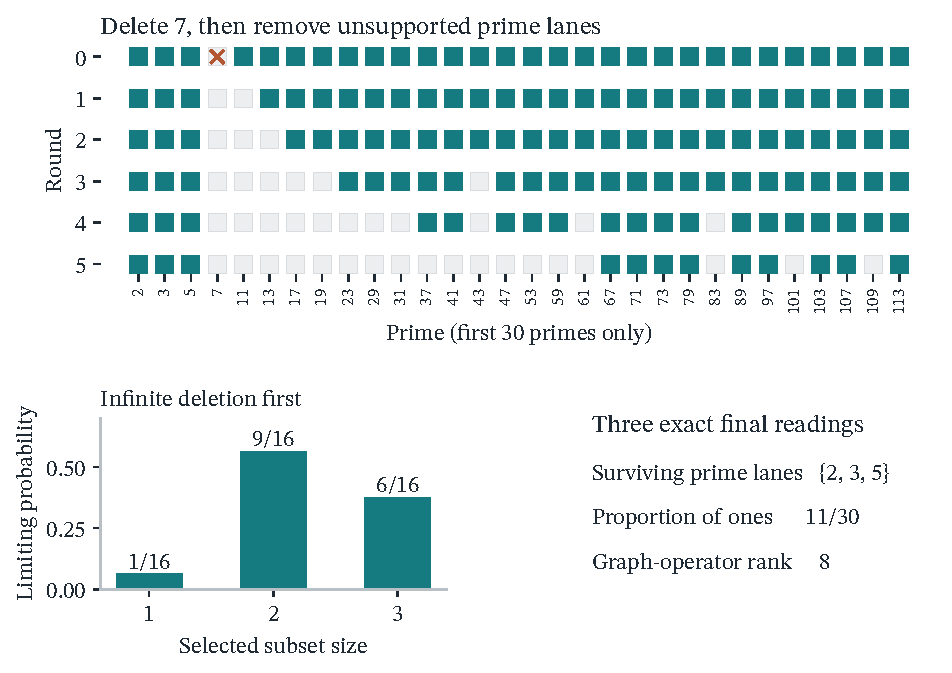
\includegraphics[width=.96\linewidth]{figures/03_delete_seven.pdf}
\caption{The upper panel follows the exact permanent-deletion rule for the first thirty primes; it is not evidence for the infinite density assertion. The lower bars give the limiting sizes of a uniformly chosen coprime subset of the $\{2,3,5\}$-smooth integers in $[2,X]$, as $X\to\infty$ after infinite deletion. The integer 1 is excluded.}
\label{fig:deletion}
\end{figure}

\subsection{An infinite spectrum becomes eight numbers}
For the last reading, give every graph vertex an independent prime
profile $\omega=(\omega_p)_{p\in\mathcal P}$: it carries $p$, meaning
$\omega_p=1$, with probability $1/p$.
Join two vertices when they share no prime in the retained set $B$.
The graph kernel and its integral operator are
\[
 G_B(\omega,\omega')=\prod_{p\in B}(1-\omega_p\omega'_p),
 \qquad
 (T_Bu)(\omega)=\int G_B(\omega,\omega')u(\omega')\,d\Prob(\omega').
\]
This operator records the graph's spectral patterns.
It is self-adjoint and Hilbert--Schmidt, and it has eigenvalues of both
signs.  It is distinct from the positive mask operator $A_g$ used in
the RH criterion.

With only $2,3,5$ retained, a vertex has eight possible relevant
profiles:
\[
 (\omega_2,\omega_3,\omega_5)\in\{0,1\}^3.
\]
Nothing else in its prime profile can affect an edge.
The final graph therefore has a finite matrix description with eight
types.  Each of the three local two-state matrices is invertible,
so all eight dimensions really occur.

Every finite round has a very different spectrum.
Let $N_{k,+}(u)$ and $N_{k,-}(u)$ count its positive and negative
eigenvalues of magnitude at least $u$.
Lemma~\ref{fin:weyl} proves
\[
 N_{k,+}(u)\sim N_{k,-}(u)\sim\frac{A_k}{2u}
 \qquad(u\downarrow0).
\]
Here $A_k>0$ measures the supply of small spectral values.
Write $K_B(4)$ for the probability that four independent profiles
form a clique when the retained restrictions are $B$.
\begin{theorem}[Infinite spectra at every finite depth]\label{fin:collapse}
Let $T_k=T_{B_k}$.  At each fixed finite depth it has infinitely many
positive and negative eigenvalues.  Their counting coefficient $A_k$
from Lemma~\ref{fin:weyl} decreases to zero.
Nevertheless $T_k$ converges in Hilbert--Schmidt norm to an operator
with exactly eight nonzero eigenvalues.  At the same time
\[
 K_{B_k}(4)\uparrow K_{\{2,3,5\}}(4)=\frac{512}{3375}.
\]
\end{theorem}

Removing prime restrictions makes such a clique more
likely, so its probability rises to $512/3375$.
At the same time $A_k$ tends to zero and the infinite spectral tail
disappears.  A fixed four-vertex experiment and the full spectrum see
different aspects of the same changing graph.

The exact tensor spectrum, the small-eigenvalue estimate, and the norm
convergence are proved in Appendix~\ref{finapp:spectrum}.
The full-prime tensor formula is due to Zagier
\cite[Appendix C]{finCoprimeChain}; here it is applied along the deletion
process.

\subsection{The initial edit can be arbitrarily late}
Deleting $7$ made the cascade easy to watch.
One can also begin arbitrarily far out in the original constant.

Let $S=\{p_i:2(i+1)\text{ has a Goldbach representation}\}$.
Choose $J\ge4$, put $r=p_J$, and initially delete the finite block
\[
 \{p_i:J<i<r\}.
\]
The same robust argument leaves density one at each finite round.
For $i\ge r$, the target $2(i+1)>2r$ cannot be made from the first
$J$ primes.  Backward dependence therefore leaves an eventual set
contained in $\{p_1,\ldots,p_J\}$.
For example, $J=4$ deletes $11$ and $13$ and leaves exactly $2,3,5,7$.

The edited lanes begin at position $p_{J+1}$.
Consequently the initial real number changes by at most
$2^{1-p_{J+1}}$.
An arbitrarily small change to the starting number can lead, under
this explicit repeated rule, to a finite eventual prime supply.

We began by hiding arithmetic answers in prime lanes.
We have now read those lanes as digits, choices and spectra.
After deleting $7$ and waiting forever, the three readings are
\[
 \frac{11}{30},\qquad \frac1{16}(1,9,6),\qquad 8.
\]
At every finite round, almost every sufficiently large prime remains.
The endpoint becomes visible only when we change the order of the
two limits.
